\section[联合观测的方法]{联合观测的方法\\Combining One-Way Observations}
单向码观测值是指一颗卫星和一台接收机间的观测值。计算一台独立接收机的位置需要4个或者更多的观测值。根据经验可知,相邻位置的误差源(比如大气延迟)是相同的。这就促使我们使用相邻两个接收机观测相同卫星的模型。此模型计算了两个接收机间的不同矢量。但是比起两个接收机位置相减的解法,这种方法并不会得到更好地结果。有时这种差分模型实际上会产生更差的结果。下面看easy4文件。

\subsection[例子4]{例子4\\easy4}
	easy4文件处理了两个接收机C/A伪距码的同步观测值。我们对两个天线的基线进行估计并在图\ref{fig:10-1}中画出了它的$(X,Y,Z)$分量。坐标变化量达到10m。因此,利用单伪距估计得到的天线位置和基线解有相同的噪声水平。这个结论仅对2000年3月2号之后的观测值有效。
	
	因此,如果对来自两个测站的同步观测数据进行处理,我们得到的基线精度是单点定位误差精度的$\sqrt{2}$倍,除非接收机观测到的伪距是负相关的。那么这种差分方法是不能改善这种情况的。
	
	只有通过使用最小二乘法程序对独立观测值(单向的)进行改正,才能提高差分向量的精度。这正是第九章提出的使用卫星地基增强系统(SBSA)的思想。当码观测值和调制在载波L1、L2上的相位观测值进行组合时,图像变化剧烈。这将在327???页做出总结。
	\begin{figure}
		\center{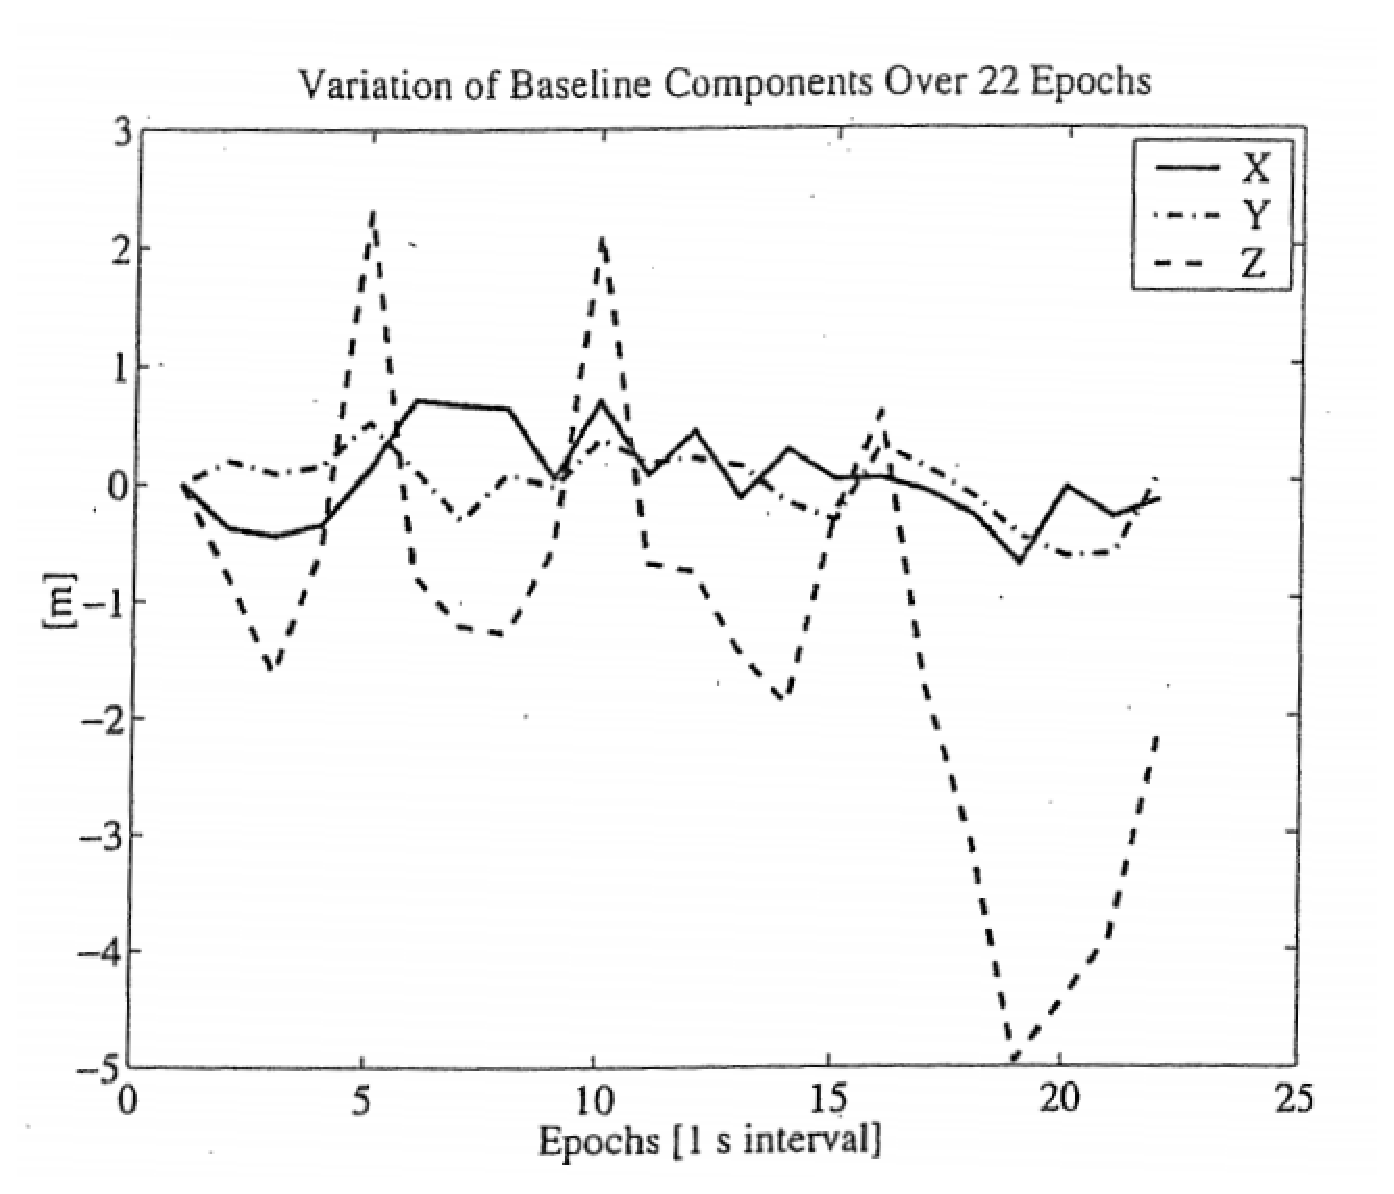
\includegraphics[width=10cm]  {TeX_files/Part03/chapter10/image/10-1.eps}}        
		\caption{ 利用两台接收机的伪距观测值估计得到的基线$(X,Y,Z)$随时间的变化}   \label{fig:10-1} 
	\end{figure}
	%CMD命令:bmeps -c inputFile.PNG outputFile.esp
	
	正如在 公式(10.2)???定义的,相位噪声$\epsilon$的标准差有几毫米,而伪距误差$\varrho$取决于接收机的质量。由于凿速率(频率的另一术语)变慢,C/A 码伪距的噪声值可以达到2$\sim$3m。P码的速率可以达到每秒1023万二进制数字或者每秒1023万位。凿速率是C/A码速率的10倍,这也暗示着P码的噪声水平在10$\sim$30cm。一个小的伪距标准差对快速固定L1,L2载波上的整周模糊度是至关重要的。P码通常是加密的,被称之为Y码。
	
	下面说明了双频接收机是如何工作的:C/A码仅调制在L1载波上,而P码既调制在L1载波上也调制在L2载波上。P码很长并且不是哥德尔序列(Gold码)。接收机利用C/A码实现与P码的同步,数据存储在导航信息中。因此,接收机只需要实现与C/A码的同步,同时解调导航信息,这与单频率接收机非常相似。在导航信息中可以找到记录一个移位寄存器当前内容的数据,这个移位寄存器用来生成P码。用这种方法就能实现P码的同步。现今的新科技允许获取P码或者是加密的Y码。更多细节详见Misra\&Enge(2006)。
	
	这章由以下组成:	
	\begin{itemize}
		\item 相位观测值;载波N的数量是未知的(模糊度)
		\item 周跳的检查;整周数N的变化
		\item 差分GPS;两台接收机
		\item 双差;两颗卫星和两台接收机
		\item 模糊度的估计;经常也是两个频率
	\end{itemize}
	

